\documentclass[usenames,dvipsnames,tikz]{standalone}
\usetikzlibrary{patterns}
%\usetikzlibrary{shapes.geometric}
%\usepackage{xcolor}
\colorlet{tBlue}{RoyalBlue!35!Cerulean}
\colorlet{tRed}{Red}
%\definecolor{tGreen}{HTML}{569909}
%\definecolor{tOrange}{HTML}{FA7602}
\usepackage{tikz}
\usepackage{standalone}
\begin{document}	
	
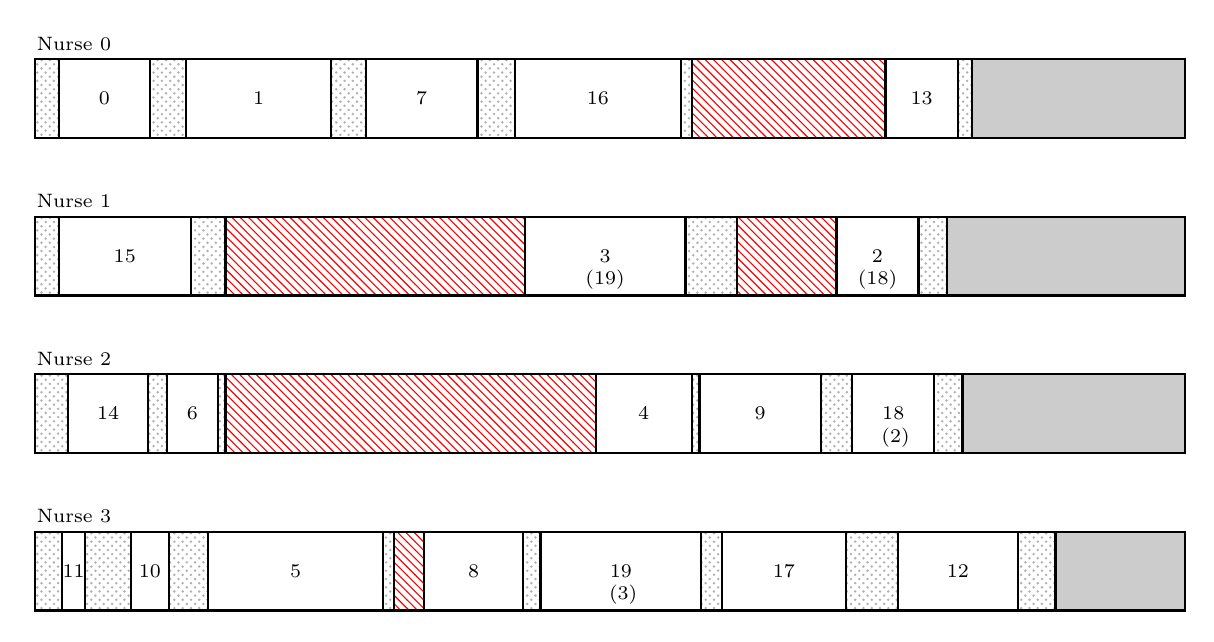
\begin{tikzpicture}
%\draw [help lines] (-1,-1) grid (15,8);

% Nurse 0
\draw [thick] (0,6) rectangle (14.6, 7);
\draw [thick, pattern = crosshatch dots, pattern color=black!30!white] (0,6) rectangle (0.30,7);
\draw [thick] (0.30,6) -- (0.30,7); % start of job 0
\draw [thick] (1.46,6) -- (1.46,7); % end of job 0
\draw [thick, pattern = crosshatch dots, pattern color=black!30!white] (1.46,6) rectangle (1.92,7);
\draw [thick] (1.92,6) -- (1.92,7); % start of job 1
\draw [thick] (3.76,6) -- (3.76,7); % end of job 1
\draw [thick, pattern = crosshatch dots, pattern color=black!30!white] (3.76,6) rectangle (4.20,7);
\draw [thick] (4.20,6) -- (4.20,7); % start of job 7
\draw [thick] (5.62,6) -- (5.62,7); % end of job 7
\draw [thick, pattern = crosshatch dots, pattern color=black!30!white] (5.62,6) rectangle (6.10,7);
\draw [thick] (6.10,6) -- (6.10,7); % start of job 16
\draw [thick] (8.20,6) -- (8.20,7); % end of job 16
\draw [thick, pattern = crosshatch dots, pattern color=black!30!white] (8.20,6) rectangle (8.34,7);
\draw [thick] (8.34,6) -- (8.34,7); % ARRIVE at job 13
\draw [thick, pattern = north west lines, pattern color=tRed] (8.34,6) rectangle (10.80,7);
\draw [thick] (10.80,6) -- (10.80,7); % start of job 13
\draw [thick] (11.72,6) -- (11.72,7); % end of job 13
\draw [thick, pattern = crosshatch dots, pattern color=black!30!white] (11.72,6) rectangle (11.90,7);
\draw [thick] (11.90,6) -- (11.90,7); % end of shift
\draw [thick, fill=black!20!white] (11.90,6) rectangle (14.6,7);

\node [right] at (-0.1,7.2) {\scriptsize{Nurse 0}};
%\node at (0.88,6.6) {\scriptsize{job}}; 
%\node at (0.88,6.35) {\scriptsize{0}};
\node at (0.88,6.5) {\scriptsize{0}};
%\node at (2.84,6.6) {\scriptsize{job}};
%\node at (2.84,6.35) {\scriptsize{1}};
\node at (2.84,6.5) {\scriptsize{1}};
%\node at (4.91,6.6) {\scriptsize{job}};
%\node at (4.91,6.35) {\scriptsize{7}};
\node at (4.91,6.5) {\scriptsize{7}};
%\node at (7.15,6.6) {\scriptsize{job}};
%\node at (7.15,6.35) {\scriptsize{16}};
\node at (7.15,6.5) {\scriptsize{16}};
%\node at (11.26,6.6) {\scriptsize{job}};
%\node at (11.26,6.35) {\scriptsize{13}};
\node at (11.26,6.5) {\scriptsize{13}};


% Nurse 1
\draw [thick] (0,4) rectangle (14.6, 5);
\draw [thick, pattern = crosshatch dots, pattern color=black!30!white] (0,4) rectangle (0.30,5);
\draw [thick] (0.30,4) -- (0.30,5); % start of job 15
\draw [thick] (1.98,4) -- (1.98,5); % end of job 15
\draw [thick, pattern = crosshatch dots, pattern color=black!30!white] (1.98,4) rectangle (2.42,5);
\draw [thick] (2.42,4) -- (2.42,5); % ARRIVE at job 3
\draw [thick, pattern = north west lines, pattern color=tRed] (2.42,4) rectangle (6.22,5);
\draw [thick] (6.22,4) -- (6.22,5); % start of job 3
\draw [thick] (8.26,4) -- (8.26,5); % end of job 3
\draw [thick, pattern = crosshatch dots, pattern color=black!30!white] (8.26,4) rectangle (8.92,5);
\draw [thick] (8.92,4) -- (8.92,5); % ARRIVE at job 2
\draw [thick, pattern = north west lines, pattern color=tRed] (8.92,4) rectangle (10.18,5);
\draw [thick] (10.18,4) -- (10.18,5); % start of job 2
\draw [thick] (11.22,4) -- (11.22,5); % end of job 2
\draw [thick, pattern = crosshatch dots, pattern color=black!30!white] (11.22,4) rectangle (11.58,5);
\draw [thick] (11.58,4) -- (11.58,5); % end of shift
\draw [thick, fill=black!20!white] (11.58,4) rectangle (14.6,5);

\node [right] at (-0.1,5.2) {\scriptsize{Nurse 1}};
%\node at (1.14,4.6) {\scriptsize{job}}; 
%\node at (1.14,4.35) {\scriptsize{15}};
\node at (1.14,4.5) {\scriptsize{15}};
%\node at (7.24,4.6) {\scriptsize{job}}; 
%\node at (7.24,4.35) {\scriptsize{3}};
\node at (7.24,4.5) {\scriptsize{3}};
\node at (7.24, 4.2) {\scriptsize{(19)}};
%\node at (10.70,4.6) {\scriptsize{job}}; 
%\node at (10.70,4.35) {\scriptsize{2}};
\node at (10.70,4.5) {\scriptsize{2}};
\node at (10.70, 4.2) {\scriptsize{(18)}};



% Nurse 2
\draw [thick] (0,2) rectangle (14.6, 3);
\draw [thick, pattern = crosshatch dots, pattern color=black!30!white] (0,2) rectangle (0.42,3);
\draw [thick] (0.42,2) -- (0.42,3); % start of job 14
\draw [thick] (1.44,2) -- (1.44,3); % end of job 14
\draw [thick, pattern = crosshatch dots, pattern color=black!30!white] (1.44,2) rectangle (1.68,3);
\draw [thick] (1.68,2) -- (1.68,3); % start of job 6
\draw [thick] (2.32,2) -- (2.32,3); % end of job 6
\draw [thick, pattern = crosshatch dots, pattern color=black!30!white] (2.32,2) rectangle (2.42,3);
\draw [thick] (2.42,2) -- (2.42,3); % ARRIVE at job 4
\draw [thick, pattern = north west lines, pattern color=tRed] (2.42,2) rectangle (7.12,3);
\draw [thick] (7.12,2) -- (7.12,3); % start of job 4
\draw [thick] (8.34,2) -- (8.34,3); % end of job 4
\draw [thick, pattern = crosshatch dots, pattern color=black!30!white] (8.34,2) rectangle (8.44,3);
\draw [thick] (8.44,2) -- (8.44,3); % start of job 9
\draw [thick] (9.98,2) -- (9.98,3); % end of job 9
\draw [thick, pattern = crosshatch dots, pattern color=black!30!white] (9.98,2) rectangle (10.38,3);
\draw [thick] (10.38,2) -- (10.38,3); % start of job 18
\draw [thick] (11.42,2) -- (11.42,3); % end of job 18
\draw [thick, pattern = crosshatch dots, pattern color=black!30!white] (11.42,2) rectangle (11.78,3);
\draw [thick] (11.78,2) -- (11.78,3); % end of shift
\draw [thick,fill=black!20!white] (11.78,2) rectangle (14.6,3);

\node [right] at (-0.1,3.2) {\scriptsize{Nurse 2}};
%\node at (0.93,2.6) {\scriptsize{job}}; 
%\node at (0.93,2.35) {\scriptsize{14}};
\node at (0.93,2.5) {\scriptsize{14}};
%\node at (2.00,2.6) {\scriptsize{job}}; 
%\node at (2.00,2.35) {\scriptsize{6}};
\node at (2.00,2.5) {\scriptsize{6}};
%\node at (7.73,2.6) {\scriptsize{job}}; 
%\node at (7.73,2.35) {\scriptsize{4}};
\node at (7.73,2.5) {\scriptsize{4}};
%\node at (9.21,2.6) {\scriptsize{job}}; 
%\node at (9.21,2.35) {\scriptsize{9}};
\node at (9.21,2.5) {\scriptsize{9}};
%\node at (10.90,2.6) {\scriptsize{job}}; 
%\node at (10.90,2.35) {\scriptsize{18}};
\node at (10.90,2.5) {\scriptsize{18}};
\node at (10.93, 2.2) {\scriptsize{(2)}};


% Nurse 3
\draw [thick] (0,0) rectangle (14.6, 1);
\draw [thick, pattern = crosshatch dots, pattern color=black!30!white] (0,0) rectangle (0.34,1);
\draw [thick] (0.34,0) -- (0.34,1); % start of job 11
\draw [thick] (0.64,0) -- (0.64,1); % end of job 11
\draw [thick, pattern = crosshatch dots, pattern color=black!30!white] (0.64,0) rectangle (1.22,1);
\draw [thick] (1.22,0) -- (1.22,1); % start of job 10
\draw [thick] (1.70,0) -- (1.70,1); % end of job 10
\draw [thick, pattern = crosshatch dots, pattern color=black!30!white] (1.70,0) rectangle (2.20,1);
\draw [thick] (2.20,0) -- (2.20,1); % start of job 5
\draw [thick] (4.42,0) -- (4.42,1); % end of job 5
\draw [thick, pattern = crosshatch dots, pattern color=black!30!white] (4.42,0) rectangle (4.56,1);
\draw [thick] (4.56,0) -- (4.56,1); % ARRIVE at job 8
\draw [thick, pattern = north west lines, pattern color=tRed] (4.56,0) rectangle (4.94,1);
\draw [thick] (4.94,0) -- (4.94,1); % start of job 8
\draw [thick] (6.20,0) -- (6.20,1); % end of job 8
\draw [thick, pattern = crosshatch dots, pattern color=black!30!white] (6.20,0) rectangle (6.42,1);
\draw [thick] (6.42,0) -- (6.42,1); % start of job 19
\draw [thick] (8.46,0) -- (8.46,1); % end of job 19
\draw [thick, pattern = crosshatch dots, pattern color=black!30!white] (8.46,0) rectangle (8.72,1);
\draw [thick] (8.72,0) -- (8.72,1); % start of job 17
\draw [thick] (10.30,0) -- (10.30,1); % end of job 17
\draw [thick, pattern = crosshatch dots, pattern color=black!30!white] (10.30,0) rectangle (10.96,1);
\draw [thick] (10.96,0) -- (10.96,1); % start of job 12
\draw [thick] (12.48,0) -- (12.48,1); % end of job 12
\draw [thick, pattern = crosshatch dots, pattern color=black!30!white] (12.48,0) rectangle (12.96,1);
\draw [thick] (12.96,0) -- (12.96,1); % end of shift
\draw [thick, fill=black!20!white] (12.96,0) rectangle (14.6,1);

\node [right] at (-0.1,1.2) {\scriptsize{Nurse 3}};
%\node at (0.49,0.6) {\scriptsize{job}}; 
%\node at (0.49,0.35) {\scriptsize{11}};
\node at (0.49,0.5) {\scriptsize{11}};
%\node at (1.46,0.6) {\scriptsize{job}}; 
%\node at (1.46,0.35) {\scriptsize{10}};
\node at (1.46,0.5) {\scriptsize{10}};
%\node at (3.31,0.6) {\scriptsize{job}}; 
%\node at (3.31,0.35) {\scriptsize{5}};
\node at (3.31,0.5) {\scriptsize{5}};
%\node at (5.57,0.6) {\scriptsize{job}}; 
%\node at (5.57,0.35) {\scriptsize{8}};
\node at (5.57,0.5) {\scriptsize{8}};
%\node at (7.44,0.6) {\scriptsize{job}}; 
%\node at (7.44,0.35) {\scriptsize{19}};
\node at (7.44 ,0.5) {\scriptsize{19}};
\node at (7.47, 0.2) {\scriptsize{(3)}};
%\node at (9.51,0.6) {\scriptsize{job}}; 
%\node at (9.51,0.35) {\scriptsize{17}};
\node at (9.51,0.5) {\scriptsize{17}};
%\node at (11.72,0.6) {\scriptsize{job}}; 
%\node at (11.72,0.35) {\scriptsize{12}};
\node at (11.72,0.5) {\scriptsize{12}};






\end{tikzpicture}
	
\end{document}

%\draw [thick] (0,6) rectangle (6.95, 7);
%\draw [thick] (0.11,6) -- (0.11,7); % start of job 10
%\draw [thick] (0.99,6) -- (0.99,7); % end of job 10
%\draw [thick] (1.07,6) -- (1.07,7); % start of job 14
%\draw [thick] (1.7,6) -- (1.7,7); % end of job 14
%\draw [thick] (1.84,6) -- (1.84,7); % start of job 3
%\draw [thick] (2.86,6) -- (2.86,7); % end of job 3
%\draw [thick] (2.93,6) -- (2.93,7); % start of job 11
%\draw [thick] (3.4,6) -- (3.4,7); % end of job 11
%\draw [thick] (3.66,6) -- (3.66,7); % start of job 17
%\draw [thick] (4.64,6) -- (4.64,7); % end of job 17
%\draw [thick] (4.76,6) -- (4.76,7); % start of job 2
%\draw [thick] (5.08,6) -- (5.08,7); % end of job 2
%\draw [thick] (5.11,6) -- (5.11,7); % start of job 0 (DS)
%\draw [thick] (6.5,6) -- (6.5,7); % end of job 0 (DS)
%\draw [thick] (6.71,6) -- (6.71,7); % end of shift


